\documentclass{article}

%Hỗ trợ gõ tiếng việt
\usepackage[utf8]{inputenc}
\usepackage[vietnam]{babel}

%Thư viện chèn ảnh
\usepackage{graphicx}
%Thư viện vẽ hình
\usepackage{picture}

\begin{document}

\section{ẢNH 1}
Xoay ảnh 30$^\circ$:
\begin{figure}[h] %Tạo vùng chứa ảnh, h nghĩa là chèn ảnh vô ngay tại vị trí câu lệnh này
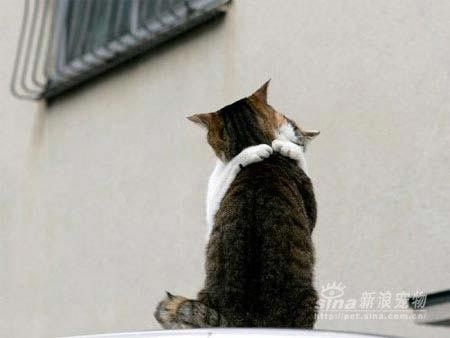
\includegraphics[angle=30, scale=0.3]{meo}
%YÊU CẦU 1: Chú thích cho ảnh 1
\end{figure}

\section{ẢNH 2}
Draw a border around a picture
\begin{figure}[h]
\setlength\fboxsep{5pt} %Khoảng cách từ khung đến đường biên của ảnh
\setlength\fboxrule{0.5pt} %Độ dầy của khung
\fbox{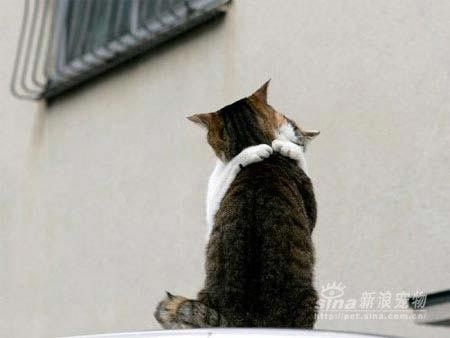
\includegraphics[scale=0.3]{meo}}
%YÊU CẦU 1: Chú thích cho ảnh 2
\end{figure}

\section{ẢNH 3}
\begin{figure}[h]
\centering
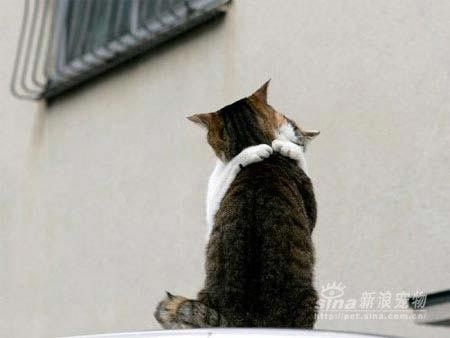
\includegraphics[scale = 0.2]{meo.jpg}
\caption{This is an image caption} %Thêm tiêu đề cho ảnh
\label{fig:meo_image} %dùng để tạo danh sách hình ảnh, tham chiếu ...
\end{figure}

\hfill\\[3cm]
\section{Vẽ hình}
\begin{picture}
%Thử thay đổi các giá trị dưới đây
(0, 0) 
\put(70, -20){object} %Đặt một đối tượng ở vị trí bất kì

\put(30, -30){\line(1, 0){5cm}} %Vẽ đoạn thẳng theo hướng vector (1,0), chiều dài 5cm, bắt đầu từ điểm có tọa độ (30, -30)

\put(35, -35){\vector(1, 0){5cm}} %Vẽ mũi tên

%Vẽ đường tròn và hình tròn
%YÊU CẦU 2: Canh cho các đường tròn có tâm ngay con mèo
\put(150,140){\circle*{10}}
\put(150,140){\circle{15}}
\put(150,140){\circle{30}}

\qbezier(0, 0)(-41, -100)(70, 11) %Vẽ đường cong

\put(50,-150){$F=\sqrt{s(s-a)(s-b)(s-c)}$}
\put(50,-100){$\displaystyle s:=\frac{a+b+c}{2}$}

\end{picture}

\end{document}